\documentclass[]{book}
\usepackage{lmodern}
\usepackage{amssymb,amsmath}
\usepackage{ifxetex,ifluatex}
\usepackage{fixltx2e} % provides \textsubscript
\ifnum 0\ifxetex 1\fi\ifluatex 1\fi=0 % if pdftex
  \usepackage[T1]{fontenc}
  \usepackage[utf8]{inputenc}
\else % if luatex or xelatex
  \ifxetex
    \usepackage{mathspec}
  \else
    \usepackage{fontspec}
  \fi
  \defaultfontfeatures{Ligatures=TeX,Scale=MatchLowercase}
\fi
% use upquote if available, for straight quotes in verbatim environments
\IfFileExists{upquote.sty}{\usepackage{upquote}}{}
% use microtype if available
\IfFileExists{microtype.sty}{%
\usepackage{microtype}
\UseMicrotypeSet[protrusion]{basicmath} % disable protrusion for tt fonts
}{}
\usepackage[margin=1in]{geometry}
\usepackage{hyperref}
\hypersetup{unicode=true,
            pdftitle={bdDwC User Guide},
            pdfauthor={Authors: Tomer Gueta and Povilas Gibas},
            pdfborder={0 0 0},
            breaklinks=true}
\urlstyle{same}  % don't use monospace font for urls
\usepackage{natbib}
\bibliographystyle{apalike}
\usepackage{color}
\usepackage{fancyvrb}
\newcommand{\VerbBar}{|}
\newcommand{\VERB}{\Verb[commandchars=\\\{\}]}
\DefineVerbatimEnvironment{Highlighting}{Verbatim}{commandchars=\\\{\}}
% Add ',fontsize=\small' for more characters per line
\usepackage{framed}
\definecolor{shadecolor}{RGB}{248,248,248}
\newenvironment{Shaded}{\begin{snugshade}}{\end{snugshade}}
\newcommand{\KeywordTok}[1]{\textcolor[rgb]{0.13,0.29,0.53}{\textbf{#1}}}
\newcommand{\DataTypeTok}[1]{\textcolor[rgb]{0.13,0.29,0.53}{#1}}
\newcommand{\DecValTok}[1]{\textcolor[rgb]{0.00,0.00,0.81}{#1}}
\newcommand{\BaseNTok}[1]{\textcolor[rgb]{0.00,0.00,0.81}{#1}}
\newcommand{\FloatTok}[1]{\textcolor[rgb]{0.00,0.00,0.81}{#1}}
\newcommand{\ConstantTok}[1]{\textcolor[rgb]{0.00,0.00,0.00}{#1}}
\newcommand{\CharTok}[1]{\textcolor[rgb]{0.31,0.60,0.02}{#1}}
\newcommand{\SpecialCharTok}[1]{\textcolor[rgb]{0.00,0.00,0.00}{#1}}
\newcommand{\StringTok}[1]{\textcolor[rgb]{0.31,0.60,0.02}{#1}}
\newcommand{\VerbatimStringTok}[1]{\textcolor[rgb]{0.31,0.60,0.02}{#1}}
\newcommand{\SpecialStringTok}[1]{\textcolor[rgb]{0.31,0.60,0.02}{#1}}
\newcommand{\ImportTok}[1]{#1}
\newcommand{\CommentTok}[1]{\textcolor[rgb]{0.56,0.35,0.01}{\textit{#1}}}
\newcommand{\DocumentationTok}[1]{\textcolor[rgb]{0.56,0.35,0.01}{\textbf{\textit{#1}}}}
\newcommand{\AnnotationTok}[1]{\textcolor[rgb]{0.56,0.35,0.01}{\textbf{\textit{#1}}}}
\newcommand{\CommentVarTok}[1]{\textcolor[rgb]{0.56,0.35,0.01}{\textbf{\textit{#1}}}}
\newcommand{\OtherTok}[1]{\textcolor[rgb]{0.56,0.35,0.01}{#1}}
\newcommand{\FunctionTok}[1]{\textcolor[rgb]{0.00,0.00,0.00}{#1}}
\newcommand{\VariableTok}[1]{\textcolor[rgb]{0.00,0.00,0.00}{#1}}
\newcommand{\ControlFlowTok}[1]{\textcolor[rgb]{0.13,0.29,0.53}{\textbf{#1}}}
\newcommand{\OperatorTok}[1]{\textcolor[rgb]{0.81,0.36,0.00}{\textbf{#1}}}
\newcommand{\BuiltInTok}[1]{#1}
\newcommand{\ExtensionTok}[1]{#1}
\newcommand{\PreprocessorTok}[1]{\textcolor[rgb]{0.56,0.35,0.01}{\textit{#1}}}
\newcommand{\AttributeTok}[1]{\textcolor[rgb]{0.77,0.63,0.00}{#1}}
\newcommand{\RegionMarkerTok}[1]{#1}
\newcommand{\InformationTok}[1]{\textcolor[rgb]{0.56,0.35,0.01}{\textbf{\textit{#1}}}}
\newcommand{\WarningTok}[1]{\textcolor[rgb]{0.56,0.35,0.01}{\textbf{\textit{#1}}}}
\newcommand{\AlertTok}[1]{\textcolor[rgb]{0.94,0.16,0.16}{#1}}
\newcommand{\ErrorTok}[1]{\textcolor[rgb]{0.64,0.00,0.00}{\textbf{#1}}}
\newcommand{\NormalTok}[1]{#1}
\usepackage{longtable,booktabs}
\usepackage{graphicx,grffile}
\makeatletter
\def\maxwidth{\ifdim\Gin@nat@width>\linewidth\linewidth\else\Gin@nat@width\fi}
\def\maxheight{\ifdim\Gin@nat@height>\textheight\textheight\else\Gin@nat@height\fi}
\makeatother
% Scale images if necessary, so that they will not overflow the page
% margins by default, and it is still possible to overwrite the defaults
% using explicit options in \includegraphics[width, height, ...]{}
\setkeys{Gin}{width=\maxwidth,height=\maxheight,keepaspectratio}
\IfFileExists{parskip.sty}{%
\usepackage{parskip}
}{% else
\setlength{\parindent}{0pt}
\setlength{\parskip}{6pt plus 2pt minus 1pt}
}
\setlength{\emergencystretch}{3em}  % prevent overfull lines
\providecommand{\tightlist}{%
  \setlength{\itemsep}{0pt}\setlength{\parskip}{0pt}}
\setcounter{secnumdepth}{5}
% Redefines (sub)paragraphs to behave more like sections
\ifx\paragraph\undefined\else
\let\oldparagraph\paragraph
\renewcommand{\paragraph}[1]{\oldparagraph{#1}\mbox{}}
\fi
\ifx\subparagraph\undefined\else
\let\oldsubparagraph\subparagraph
\renewcommand{\subparagraph}[1]{\oldsubparagraph{#1}\mbox{}}
\fi

%%% Use protect on footnotes to avoid problems with footnotes in titles
\let\rmarkdownfootnote\footnote%
\def\footnote{\protect\rmarkdownfootnote}

%%% Change title format to be more compact
\usepackage{titling}

% Create subtitle command for use in maketitle
\newcommand{\subtitle}[1]{
  \posttitle{
    \begin{center}\large#1\end{center}
    }
}

\setlength{\droptitle}{-2em}

  \title{\texttt{bdDwC} User Guide}
    \pretitle{\vspace{\droptitle}\centering\huge}
  \posttitle{\par}
    \author{Authors: Tomer Gueta and Povilas Gibas}
    \preauthor{\centering\large\emph}
  \postauthor{\par}
      \predate{\centering\large\emph}
  \postdate{\par}
    \date{built on2018-11-28 - for bdDwC v0.1.21}

\usepackage{booktabs}

\usepackage{amsthm}
\newtheorem{theorem}{Theorem}[chapter]
\newtheorem{lemma}{Lemma}[chapter]
\theoremstyle{definition}
\newtheorem{definition}{Definition}[chapter]
\newtheorem{corollary}{Corollary}[chapter]
\newtheorem{proposition}{Proposition}[chapter]
\theoremstyle{definition}
\newtheorem{example}{Example}[chapter]
\theoremstyle{definition}
\newtheorem{exercise}{Exercise}[chapter]
\theoremstyle{remark}
\newtheorem*{remark}{Remark}
\newtheorem*{solution}{Solution}
\begin{document}
\maketitle

{
\setcounter{tocdepth}{1}
\tableofcontents
}
\chapter*{Introduction}\label{introduction}
\addcontentsline{toc}{chapter}{Introduction}

\texttt{bdDwC} is a R package that supplies an interactive Shiny app and
a set of functions for standardizing field names in compliance to the
Darwin Core (DwC) format. \texttt{bdDwC} is a key element in the
\texttt{bdverse}-- a collection of tools, that form a general framework
for facilitating biodiversity science in R.

\begin{figure}
\centering
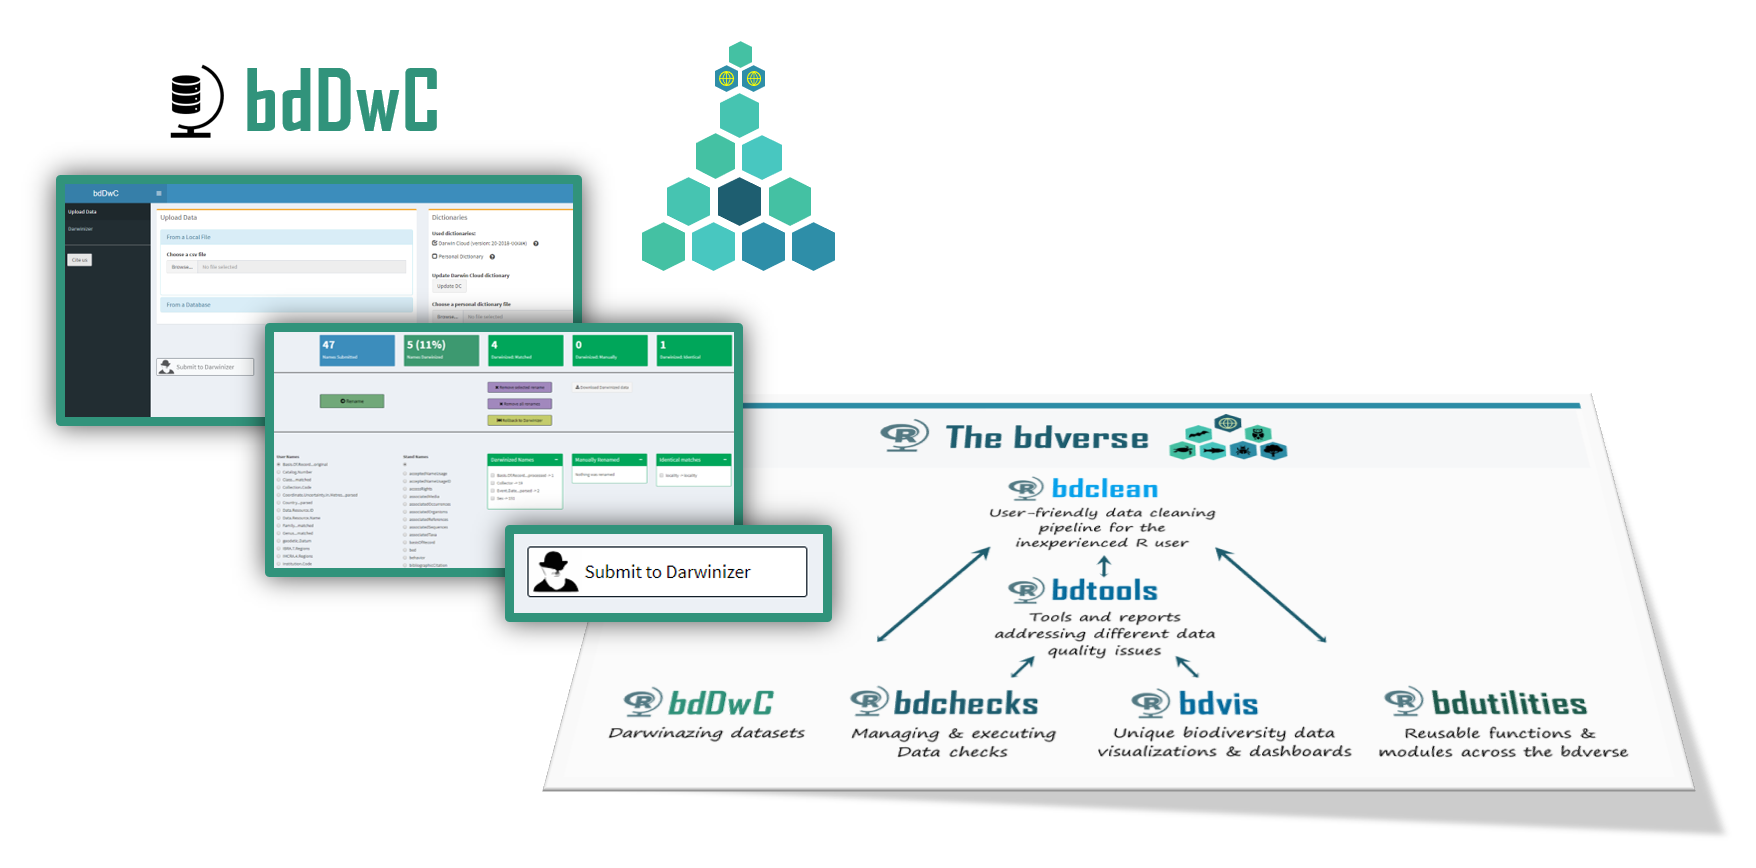
\includegraphics{img/bdDwC_bdverse.png}
\caption{bdDwC in the bdverse}
\end{figure}

\subsubsection*{What is the Darwin Core
standard?}\label{what-is-the-darwin-core-standard}
\addcontentsline{toc}{subsubsection}{What is the Darwin Core standard?}

Darwin Core (DwC) is a global standard for publishing biodiversity data,
whose goal is to facilitate the sharing of biodiversity information, by
providing identifiers, labels, and definitions \citep{DwC-paper}. DwC
was established as an evolving community-developed standard, by the
Biodiversity Information Standards Working Group (www.tdwg.org). DwC is
a library of definitions of common biodiversity data terms, each of
which represents a field within the database. There are around 200 such
fields (not including DwC extensions); a full set of the DwC terms with
their descriptions is available in the Quick Reference Guide
(\url{http://rs.tdwg.org/dwc/terms}). For more information see section
\protect\hyperlink{learn-more-about-darwin-core}{6}.

\subsubsection*{\texorpdfstring{Why it's important to ``Darwinize'' a
dataset}{Why it's important to Darwinize a dataset}}\label{why-its-important-to-darwinize-a-dataset}
\addcontentsline{toc}{subsubsection}{Why it's important to ``Darwinize''
a dataset}

Running the Darwinizer enables you to standardize many field names in
your dataset -- and that allows the \texttt{bdverse} to handle data from
various biodiversity portals seamlessly, and lets you enjoy all of
\texttt{bdvers} features, regardless of publishers variation in field
names.

\subsubsection*{Fundings}\label{fundings}
\addcontentsline{toc}{subsubsection}{Fundings}

\begin{figure}
\centering

\includegraphics{img/ISF.png}
\caption{}
\end{figure}

\href{https://summerofcode.withgoogle.com/\%20target=\%22_blank\%22}{
\includegraphics{img/GSoC.png}}

\begin{itemize}
\tightlist
\item
  See the GSoC project idea page
\end{itemize}

\chapter{\texorpdfstring{Installing
\texttt{bdDwC}}{Installing bdDwC}}\label{installing-bddwc}

\begin{center}\rule{0.5\linewidth}{\linethickness}\end{center}

\section{Stable version from CRAN}\label{stable-version-from-cran}

\begin{Shaded}
\begin{Highlighting}[]
\KeywordTok{install.packages}\NormalTok{(}\StringTok{"bdDwC"}\NormalTok{)}
\end{Highlighting}
\end{Shaded}

\section{Development version from
GitHub}\label{development-version-from-github}

Windows users install
\href{https://cran.r-project.org/bin/windows/Rtools/}{Rtools} first.

\begin{Shaded}
\begin{Highlighting}[]
\KeywordTok{install.packages}\NormalTok{(}\StringTok{"devtools"}\NormalTok{)}
\NormalTok{devtools}\OperatorTok{::}\KeywordTok{install_github}\NormalTok{(}\StringTok{"bd-R/bdDwC"}\NormalTok{)}
\end{Highlighting}
\end{Shaded}

\section{Possible problems \&
solutions}\label{possible-problems-solutions}

\textbf{{{[} TBA {]}}}

\subsection{???}\label{section}

TBA

\subsection{????}\label{section-1}

TBA

\chapter{The shiny app}\label{the-shiny-app}

\begin{center}\rule{0.5\linewidth}{\linethickness}\end{center}

\section{Launching the app}\label{launching-the-app}

\begin{Shaded}
\begin{Highlighting}[]
\KeywordTok{library}\NormalTok{(bdDwC) }\CommentTok{# Laod package library}
\KeywordTok{runDwC}\NormalTok{() }\CommentTok{# Launch the app}
\end{Highlighting}
\end{Shaded}

\section{App overview}\label{app-overview}

\begin{figure}
\centering
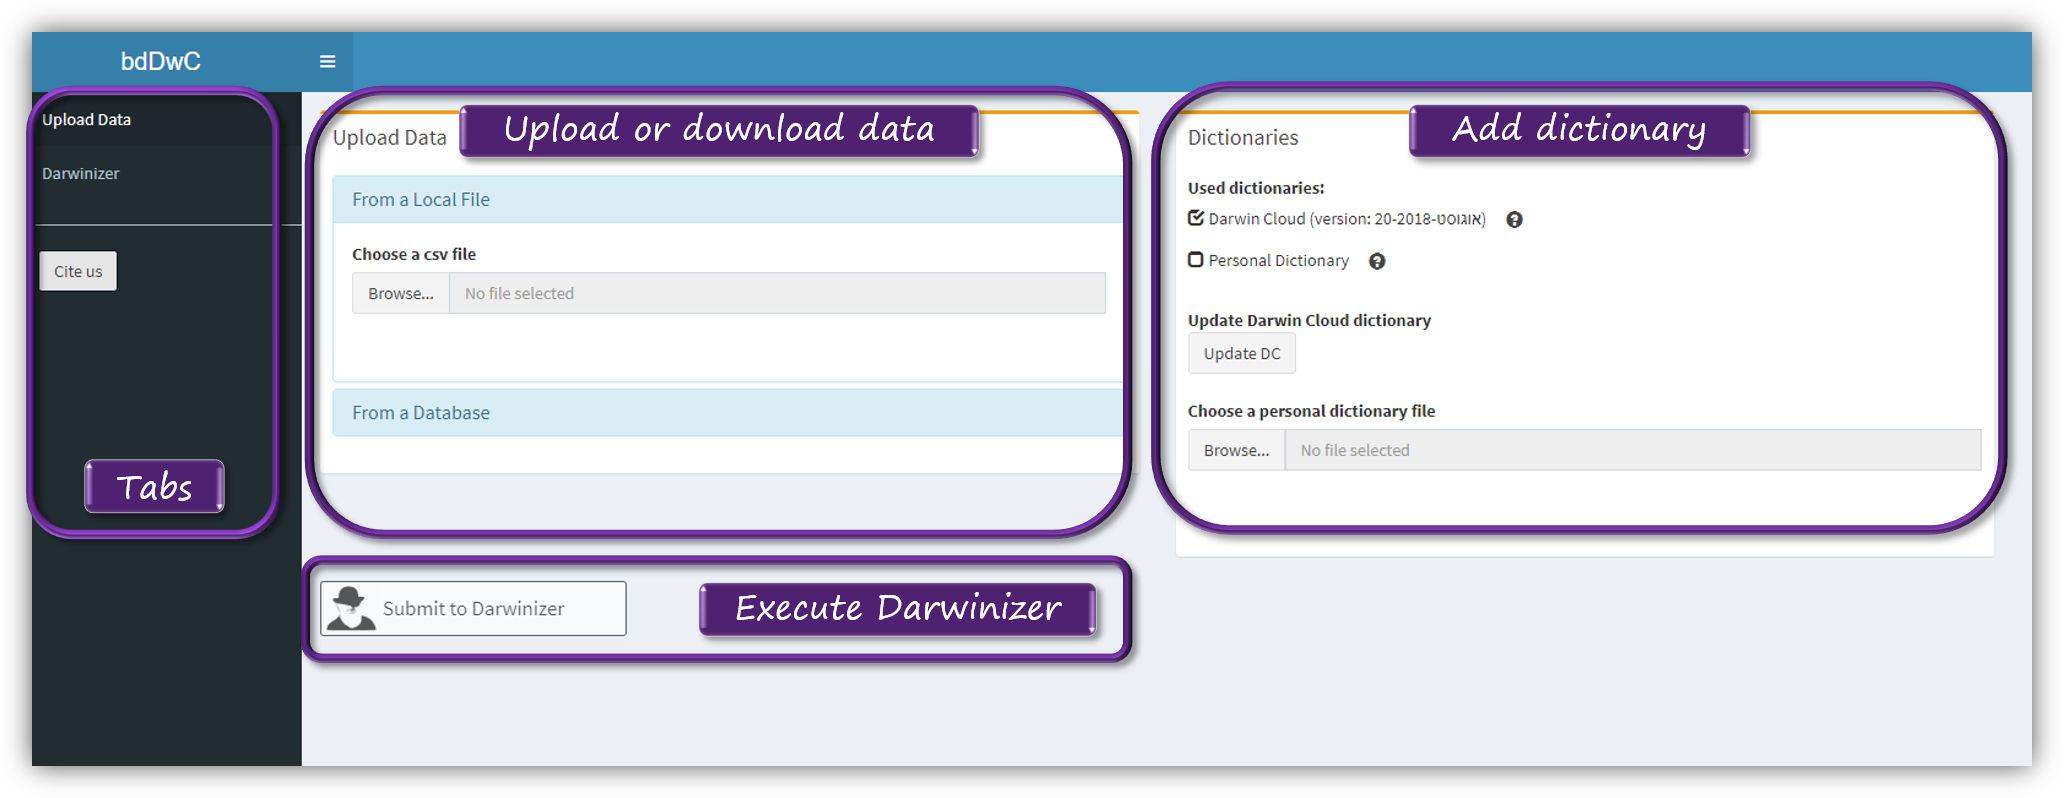
\includegraphics{img/bdDwC_Getting_started.png}
\caption{bdDwC App Overview}
\end{figure}

In the first screen, you'll need to load your biodiversity data; choose
dictionary and run the Darwinizer. There are two options, form a file on
your computer, of fetch from a web based data provider.

\section{Data upload}\label{data-upload}

\subsection{From a local file}\label{from-a-local-file}

A CSV file or a Darwin Core Archive (DwC-A) zip file can be uploaded.

\begin{figure}
\centering
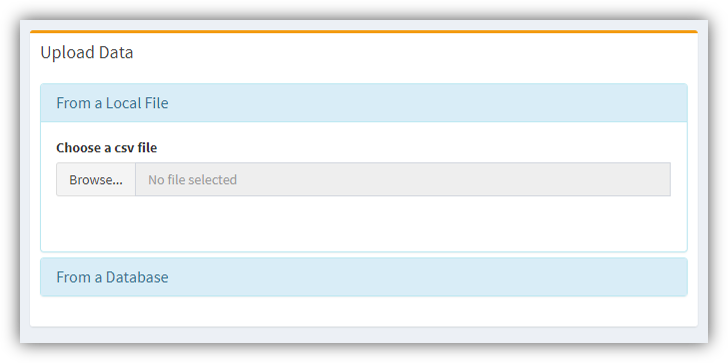
\includegraphics{img/bdDwC_Up-local_file.png}
\caption{Data upload from a local file}
\end{figure}

\subsection{From an online database}\label{from-an-online-database}

Also, data can be retrieved directly from various online biodiversity
databases. You need only to:

\begin{itemize}
\tightlist
\item
  Select the database
\item
  Specify the desired scientific name.
\item
  Specify the number of records (upper limit of 50,000).
\item
  Check the box if records must have coordinates.
\item
  Wait for data to be downloaded.
\end{itemize}

\begin{figure}
\centering
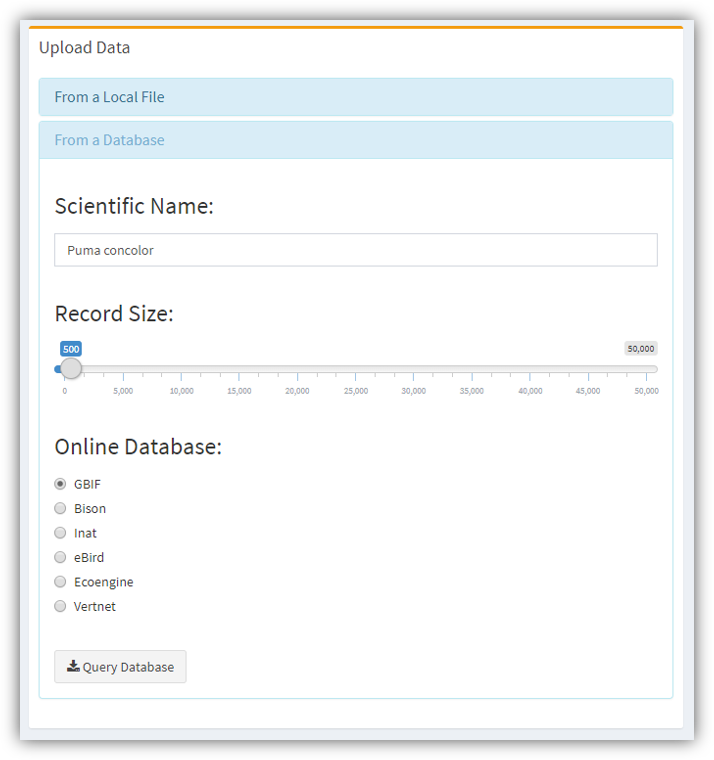
\includegraphics{img/bdDwC_Up-database.png}
\caption{Data upload from online biodiversity databases}
\end{figure}

\section{Dictionaries}\label{dictionaries}

A dictionary is a key component when Darwinizing a dataset. It's
basically a lookup table that lists a possible variation of field name
and it corresponding DwC name.

\hypertarget{the-darwin-cloud-dictionary}{\subsection{The Darwin Cloud
dictionary}\label{the-darwin-cloud-dictionary}}

The Darwin Cloud dictionary \citep{DarwinCloud}, is a lookup table that
accumulates different variations in DwC field names from different
publishers. This valuable and critical dictionary was created and is
maintained by the Kurator project
(\url{http://kurator.acis.ufl.edu/kurator-web/}), which provides
workflow tools for data quality improvement of biodiversity data, via a
user-friendly web interface. The development of bdDwC was inspired by
Kurator's own Darwinizer.

\subsubsection*{Updating the Darwin Cloud
dictionary}\label{updating-the-darwin-cloud-dictionary}
\addcontentsline{toc}{subsubsection}{Updating the Darwin Cloud
dictionary}

It's recommended to update the Darwin Cloud dictionary file. This can be
done easily by clicking the \textbf{Update DC} button.

\begin{figure}
\centering
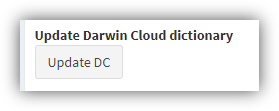
\includegraphics{img/bdDwC_update-DC.png}
\caption{Updating the Darwin Cloud dictionary}
\end{figure}

\subsection{Custom dictionary}\label{custom-dictionary}

It's also possible to add your own dictionary by creating a CSV file
with two columns, one for the Field Names and one for the Standard
Names. After uploading the custom disctionary, we need to specify which
field denotes the `User fierld names' and which is the `Standard (DwC)
field names'.

\begin{figure}
\centering
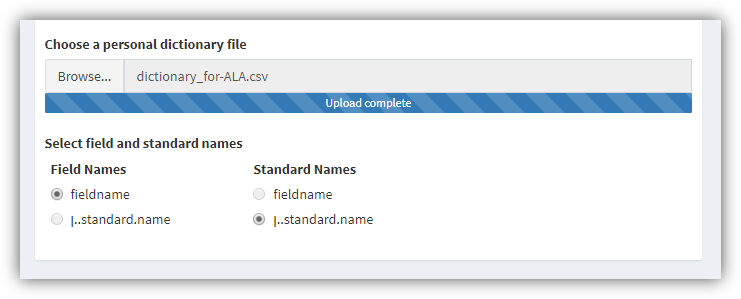
\includegraphics{img/bdDwC_personal_dictionary.png}
\caption{Uploading your own dictionary}
\end{figure}

\section{Darwinizing your dataset}\label{darwinizing-your-dataset}

Once a dataset is uploaded, the `Submit to Darwinizer' button is
activated, Clicking it will begin the interactive `Darwinize the
dataset' process.

\begin{figure}
\centering
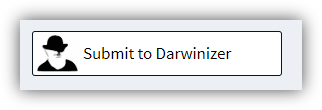
\includegraphics{img/bdDwC_Submit.png}
\caption{Submit to Darwinizer button}
\end{figure}

\section{Darwinizer results}\label{darwinizer-results}

\subsection{Results page overwiew}\label{results-page-overwiew}

\begin{figure}
\centering
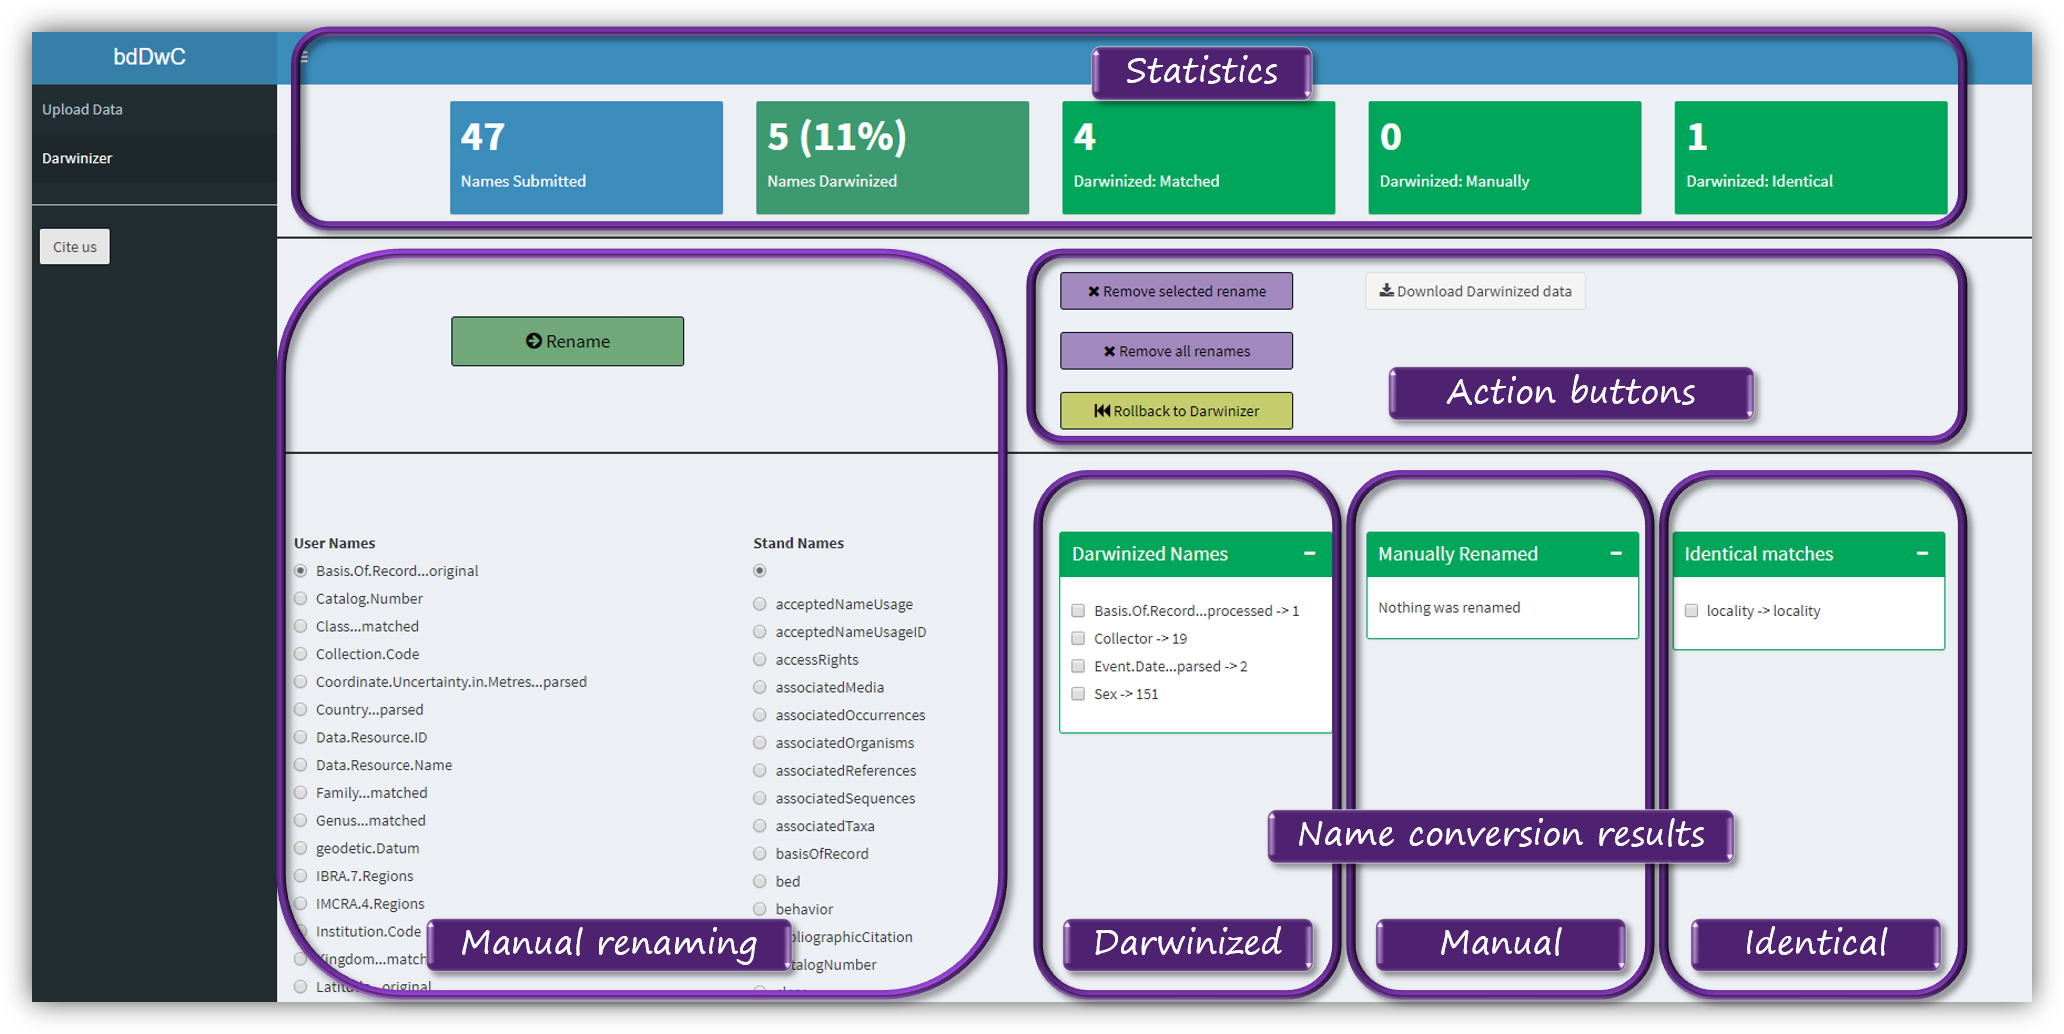
\includegraphics{img/bdDwC_Darwinizer_results.png}
\caption{Darwinizer results}
\end{figure}

Manually renaming field names can be done very easily, just choose the
two corresponding fields and click the Rename button.

\begin{figure}
\centering
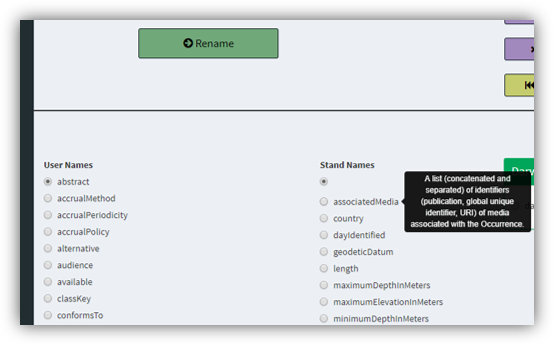
\includegraphics{img/bdDwC_Manual_rename.png}
\caption{Manually renaming fields}
\end{figure}

Hovering over a DwC standard name will display its description.

\section{Download your Darwinized
data}\label{download-your-darwinized-data}

\section{Closing the app}\label{closing-the-app}

Just close the app browser tab, and the R session will be terminated. To
reopen it run in the R Console \texttt{runDwC()}.

\section{References}\label{references}

\chapter{Command line operations}\label{command-line-operations}

\begin{center}\rule{0.5\linewidth}{\linethickness}\end{center}

\section{Load package}\label{load-package}

Load the \texttt{bdDwC} package

\begin{Shaded}
\begin{Highlighting}[]
    \KeywordTok{library}\NormalTok{(bdDwC)}
\end{Highlighting}
\end{Shaded}

\section{Darwinizing a dataset}\label{darwinizing-a-dataset}

\texttt{bdDwC} contains Indian Reptile dataset
\texttt{bdDwC:::dataReptiles}.

The function to Darwinize a dataset is\texttt{darwinizeNames} (replace
\texttt{bdDwC:::dataReptiles} with wanted dataset):

\begin{Shaded}
\begin{Highlighting}[]
\NormalTok{result <-}\StringTok{ }\KeywordTok{darwinizeNames}\NormalTok{(}\DataTypeTok{dataUser =}\NormalTok{ bdDwC}\OperatorTok{:::}\NormalTok{dataReptiles,}
                            \DataTypeTok{dataDWC   =}\NormalTok{ bdDwC}\OperatorTok{:::}\NormalTok{dataDarwinCloud}\OperatorTok{$}\NormalTok{data)}
\end{Highlighting}
\end{Shaded}

You can replace \texttt{bdDwC:::dataReptiles} with your dataset

Rename your dataset field names to Darwinized names using
\texttt{renameUserData}:

\begin{Shaded}
\begin{Highlighting}[]
\KeywordTok{renameUserData}\NormalTok{(bdDwC}\OperatorTok{:::}\NormalTok{dataReptiles, result)}
\end{Highlighting}
\end{Shaded}

\section{\texorpdfstring{Updating
\protect\hyperlink{the-darwin-cloud-dictionary}{the Darwin Cloud
dictionary}}{Updating the Darwin Cloud dictionary}}\label{updating-the-darwin-cloud-dictionary-1}

To get newest version of Darwin Cloud Data run:

\begin{Shaded}
\begin{Highlighting}[]
\KeywordTok{downloadCloudData}\NormalTok{()}
\end{Highlighting}
\end{Shaded}

which will download data from the remote repository and extract field
and standard names.

\chapter{Examples}\label{examples}

\begin{center}\rule{0.5\linewidth}{\linethickness}\end{center}

\textbf{{{[} TBA {]}}}

\chapter{Getting your feedback}\label{getting-your-feedback}

\begin{center}\rule{0.5\linewidth}{\linethickness}\end{center}

Loading\ldots{}

\section{Report a bug}\label{report-a-bug}

Submit an issue at \url{https://github.com/bd-R/bdDwC/issues}

\section{Contribute}\label{contribute}

Contribute: \url{https://github.com/bd-R/bdDwC}

Join: \url{https://bd-r-group.slack.com}

\chapter{\texorpdfstring{\texttt{bdDwC}
citation}{bdDwC citation}}\label{bddwc-citation}

\begin{center}\rule{0.5\linewidth}{\linethickness}\end{center}

\begin{Shaded}
\begin{Highlighting}[]
\KeywordTok{citation}\NormalTok{(}\StringTok{"bdDwC"}\NormalTok{)}
\end{Highlighting}
\end{Shaded}

\begin{verbatim}
## 
## To cite package 'bdDwC' in publications use:
## 
##   Povilas Gibas, Tomer Gueta, Vijay Barve, Thiloshon Nagarajah and
##   Yohay Carmel (2018). bdDwC: field names conversion to Darwin
##   Core (DwC) format. R package version 0.1.21.
##   https://github.com/bd-R/bdDwC
## 
## A BibTeX entry for LaTeX users is
## 
##   @Manual{,
##     title = {bdDwC: field names conversion to Darwin Core (DwC) format},
##     author = {Povilas Gibas and Tomer Gueta and Vijay Barve and Thiloshon Nagarajah and Yohay Carmel},
##     year = {2018},
##     note = {R package version 0.1.21},
##     url = {https://github.com/bd-R/bdDwC},
##   }
\end{verbatim}

\hypertarget{learn-more-about-darwin-core}{\chapter{Learn more about
Darwin Core}\label{learn-more-about-darwin-core}}

\begin{center}\rule{0.5\linewidth}{\linethickness}\end{center}

\begin{itemize}
\item
  \textbf{\href{https://github.com/tdwg/dwc-qa}{The Darwin Core
  Questions \& Answers Site}}
\item
  \textbf{\href{https://github.com/tdwg/dwc-qa/wiki/Webinars}{Darwin
  Core Hour webinar series}}
\item
  \textbf{\href{https://github.com/tdwg/dwc-qa/wiki}{The Darwin Core
  Questions \& Answers wiki}}
\item
  \textbf{\href{https://www.gbif.org/darwin-core}{GBIF: What is Darwin
  Core, and why does it matter?}}
\item
  \textbf{\href{https://doi.org/10.1371/journal.pone.0029715}{Darwin
  Core: An Evolving Community-Developed Biodiversity Data Standard}
  \citep{DwC-paper} }
\end{itemize}

\subsubsection*{References}\label{references-1}
\addcontentsline{toc}{subsubsection}{References}

\bibliography{bib/DarwinCloud.bib,bib/DwC-paper.bib}


\end{document}
